\documentclass[a4paper]{article}
\usepackage{graphicx}
\usepackage{listings}
\usepackage[utf8]{inputenc}
\usepackage{caption}
\usepackage{multirow}
\usepackage{pdflscape}
\usepackage{afterpage}

\title{Trabajo Práctico Nro. 3:\\``Sistema de llenado\\y vaciado de un tanque''}
\author{Amodey, Leandro - leandroamodey@gmail.com
\and Monti, Matías - matiasmonti@hotmail.com
\and Quinteros, Fernando - lordfers@gmail.com
\and Araneda, Alejandro – eloscurodeefeso@hotmail.com}
\date{1er. Cuatrimestre 2020\\Jueves, 25 de Junio}

\def\teacher{Ing. Jorge H. Doorn
\and Ing. Matías Presso}

\captionsetup{justification=centering,labelsep=period,font={small},%
labelfont=bf,textfont=it}
\renewcommand{\figurename}{Figura}
\renewcommand{\abstractname}{Resumen}
\renewcommand{\refname}{Referencias}
\let\originalcite\cite
\renewcommand{\cite}[2][]{\textsuperscript{\originalcite{#2}}}
\makeatletter\let\@afterindentfalse\@afterindenttrue\makeatother
\let\originalappendix\appendix
\renewcommand{\appendix}{%
    \newpage\originalappendix\pagenumbering{gobble}%
    \renewcommand\thesection{Anexo \Alph{section}}
    \setcounter{secnumdepth}{1}
}
\setcounter{secnumdepth}{0}

\begin{document}

\begin{titlepage}\renewcommand\and\par\centering\makeatletter
    
\includegraphics{logo.png}\par
    {\Large Ingeniería en Computación \par}\vspace{0.5cm}
    {\LARGE Laboratorio de Microprocesadores \par}\vfill
    {\huge \@title \par}\vfill
    Grupo 2:\par
    \@author\vfill
    Práctica entregada:\par
    \@date\vfill
    Docentes:\par
    \teacher\vspace{1cm}\makeatother
\end{titlepage}

\begin{abstract}

    En el presente trabajo realizamos el análisis y diseño de la
    implementacion de un sistema que se ocupa del llenado y vaciado 
    de un tanque mediante el uso de microcontroladores y otros 
    componentes electrónicos.

\end{abstract}

\section{Introducción}

Para este trabajo utilizaremos los conocimientos adquiridos en los 
trabajos anteriores y otras materias sumando nuevas herramientas las
 cuales fuimos investigando a medida que realizamos el mismo, a
 continuación iremos describiendo las que consideremos más importantes.

\subsubsection*{Sensor}

En primer lugar como la consigna aclara que tanto para vaciar y llenar 
el tanque este debe estar entre ciertos niveles de agua debemos contar 
con una herramienta que nos permita saber la cantidad actual del tanque,
 para esto utilizaremos un sensor del nivel de agua.

Este sensor se alimenta a 5V o a 3,3V, el pin S nos dará un valor 
analógico de manera que usaremos el pin S conectándolo como entrada
 analógica, el valor que leamos será mayor en función de la superficie 
del sensor este cubierto de agua. Esto se debe a que el agua se comporta 
como un conductor, teniendo en cuenta que el agua que usemos en nuestros 
depósitos no será agua pura (H2O), ya que de por si el agua no es 
conductora.

\subsubsection*{Conversor digital analógico/escalera de resistencias}

Señales digitales: Son variables eléctricas con dos niveles bien 
diferenciados que se alternan en el tiempo transmitiendo información
 según un código previamente acordado.

Señales analógicas: Son variables eléctricas que evolucionan en el 
tiempo en forma análoga a alguna variable física.

Utilizaremos un conversor o convertidor digital analógico (DAC) R-2R 
como el que se muestra el la Figura \ref{fig:conversor}, que suma 
varias señales digitales binarias de acuerdo al peso de cada 
una dando como resultado una señal de corriente o tensión analógica.

\begin{figure}[h]\centering
    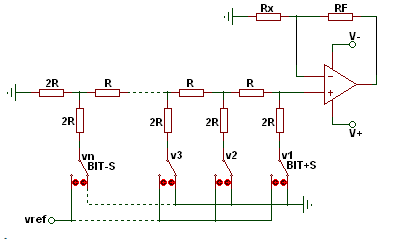
\includegraphics[height=4cm]{conversor.png}
    \caption{convertidor digital analógico (DAC) R-2R}
    \label{fig:conversor}
\end{figure}

Se llama R-2R por la forma de escalera que tiene el circuito y por 
los valores que toman las resistencias R y 2R, gracias a esto al pic 
ingresa un valor binario el cual luego será utilizado para hacer 
comparaciones en la lógica del programa, además presenta algunas 
ventajas como la alta velocidad de conversión o el funcionamiento 
sencillo, mientras que por otro lado los valores de las resistencias 
tienen que ser precisos, sobre todo los de las resistencias de los
 bits MSB (Most Significant Bit) además de que son necesarias muchas
 resistencias. El R-2R brinda un voltaje a la salida que va entre 0
 a 5 V si se considerada que las entradas digitales pueden brindar 
únicamente esos dos valores y tendrán $2^n$ valores analógicos 
posibles.

\subsubsection*{Bombas de Agua}

Una bomba de agua es una máquina hidráulica que permite incrementar 
la energía cinética de un caudal de agua. Las bombas hidráulicas son 
elementos ampliamente conocidos y empleados
 en la industria desde antaño, y constituyen toda una rama de la 
 técnica. Existe una gran variedad de bombas, que abarcan un amplio 
 rango de potencias y características hidráulicas.

Independientemente de sus características o potencia, siempre podemos 
controlar un equipo de bombeo mediante un procesador, siendo de hecho 
frecuente que estén controlados por un autómata. Arduino, por 
supuesto, no es una excepción, y podemos encender cualquier tipo de 
bomba de agua mediante las salidas digitales y el uso de un MOSFET o 
una salida por relé.

\subsubsection*{Relé}

Un relé es un interruptor accionado eléctricamente. Muchos relé 
utilizan un electroimán para operar mecánicamente un interruptor, 
pero otros principios de funcionamiento también se utilizan los 
relés de estado sólido. Los relés se utilizan cuando es necesario 
para controlar un circuito por una señal de baja potencia (con 
aislamiento eléctrico completo entre el control y los circuitos 
controlados), o cuando varios circuitos deben ser controlados por 
una señal.

\begin{figure}[h]\centering
    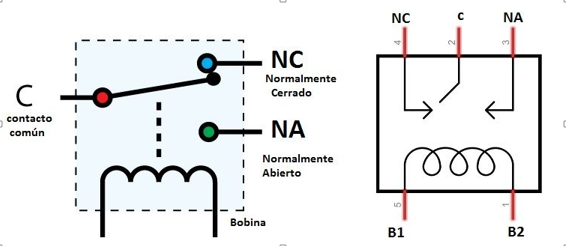
\includegraphics[height=4cm]{rele.png}
    \caption{Relé}
    \label{fig:Rele}
\end{figure}

En la Figura \ref{fig:Rele} se ve un esquema con el funcionamiento 
del Relé, al meter corriente por la bobina los contactos abiertos 
se cierran y los cerrados se abren.

\subsubsection*{Optoacoplador}

El propósito principal de un optoacoplador es proteger al circuito 
de salida frente a picos de voltajes o tensiones elevadas en su 
entrada que pueden dañar al otro circuito. Un optoacoplador 
contiene, por lo general, un LED que convierte la señal eléctrica 
de entrada en luz y un sensor que detecta la luz del LED.

\begin{figure}[h]\centering
    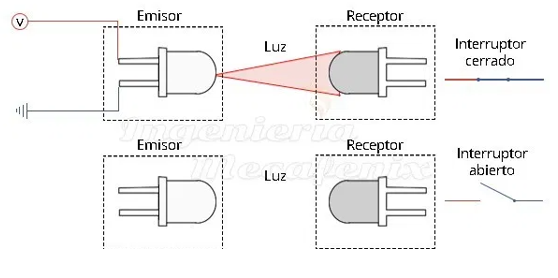
\includegraphics[height=4cm]{Optoacoplador.png}
    \caption{Optoacoplador}
    \label{fig:Optoacoplador}
\end{figure}

En la Figura \ref{fig:Optoacoplador} se muestra como funciona el 
Optoacoplador en sus dos estados. Como se observa, el mismo 
cuenta con un emisor y un receptor. El emisor es 
un led infrarrojo que manda un haz de luz hacia el receptor que 
normalmente es un fototransistor, cuando este dispositivo capta 
la señal actúa como un interruptor cerrado y cuando se interrumpe 
actúa como un interruptor abierto.

\section{Descripción de la Práctica}

\afterpage{
\begin{landscape}
    \begin{table}[p]\centering
        \begin{tabular}{|c|c|c|c|c|cccc|c|}
            \hline
            \multirow{2}{*}{Descripción}      & \multirow{2}{*}{Marca}   & \multirow{2}{*}{Modelo} & \multicolumn{2}{c|}{Alimentación / Control}                                                                                 & \multicolumn{4}{c|}{Respuesta}                                                                                                                                                                                                                                                                                                & \multirow{2}{*}{\begin{tabular}[c]{@{}c@{}}Precio\\ (pesos)\end{tabular}} \\ \cline{4-5}
                                              &                          &                         & \begin{tabular}[c]{@{}c@{}}Tensión\\ (voltios)\end{tabular} & \begin{tabular}[c]{@{}c@{}}Corriente\\ (amperes)\end{tabular} &                                                                                  &                                                                                  &                                                                                            &                                                            &                                                                           \\ \hline
            \multirow{2}{*}{Bomba periférica} & \multirow{2}{*}{Fluvial} & \multirow{2}{*}{Nero}   & \multirow{2}{*}{220 V}                                      & \multirow{2}{*}{2,4 A}                                        & \multicolumn{1}{c|}{\begin{tabular}[c]{@{}c@{}}Potencia\\ (vatios)\end{tabular}} & \multicolumn{1}{c|}{\begin{tabular}[c]{@{}c@{}}Altura\\ (metros)\end{tabular}}   & \multicolumn{1}{c|}{\begin{tabular}[c]{@{}c@{}}Caudal\\ (litros/\\ segundos)\end{tabular}} & \begin{tabular}[c]{@{}c@{}}Succión\\ (metros)\end{tabular} & \multirow{2}{*}{\$ 2.700}                                                 \\ \cline{6-9}
                                              &                          &                         &                                                             &                                                               & \multicolumn{1}{c|}{0,37 KW}                                                     & \multicolumn{1}{c|}{32 m}                                                        & \multicolumn{1}{c|}{0,55 l/s}                                                              & 9 m                                                        &                                                                           \\ \hline
            \multirow{2}{*}{Rele}             & \multirow{2}{*}{Songle}  & \multirow{2}{*}{SRD}    & \multirow{2}{*}{5 V}                                        & \multirow{2}{*}{90 mA}                                        & \multicolumn{2}{c|}{\begin{tabular}[c]{@{}c@{}}Tension\\ (voltios)\end{tabular}}                                                                                    & \multicolumn{2}{c|}{\begin{tabular}[c]{@{}c@{}}Corriente\\ (amperes)\end{tabular}}                                                                      & \multirow{2}{*}{\$ 150}                                                   \\ \cline{6-9}
                                              &                          &                         &                                                             &                                                               & \multicolumn{2}{c|}{240 V}                                                                                                                                          & \multicolumn{2}{c|}{10 A}                                                                                                                               &                                                                           \\ \hline
            \multirow{2}{*}{Transistor BJT}   & \multirow{2}{*}{ON}      & \multirow{2}{*}{BC547}  & \multirow{2}{*}{0,6V}                                       & \multirow{2}{*}{1 mA}                                         & \multicolumn{1}{c|}{\begin{tabular}[c]{@{}c@{}}Potencia\\ (vatios)\end{tabular}} & \multicolumn{1}{c|}{\begin{tabular}[c]{@{}c@{}}Tension\\ (voltios)\end{tabular}} & \multicolumn{1}{c|}{\begin{tabular}[c]{@{}c@{}}Corriente\\ (amperes)\end{tabular}}         & \begin{tabular}[c]{@{}c@{}}Ganancia\\ ó hFE\end{tabular}   & \multirow{2}{*}{\$ 10}                                                    \\ \cline{6-9}
                                              &                          &                         &                                                             &                                                               & \multicolumn{1}{c|}{500 mW}                                                      & \multicolumn{1}{c|}{45 V}                                                        & \multicolumn{1}{c|}{100 mA}                                                                & 110                                                        &                                                                           \\ \hline
        \end{tabular}
        \caption{Componentes utilizados en el diseño de la aplicación}
        \label{tab:componentes}
    \end{table}
\end{landscape}}

\subsection{Enunciado}

A continuación transcribimos el enunciado original de la práctica del
que se extraen los requerimientos para el desarrollo.

\begin{quotation}

    \begin{center}\textit{\textbf{%
        Taller de Microprocesadores: Trabajo Practico Nro. 3%
    }}\end{center}\vspace{1em}

    Diseñar un sistema que permita llenar y vaciar un tanque de líquido 
    con dos bombas independientes. 

    El inicio de llenado del tanque debe realizarlo mediante un botón 
    (o señal digital externa ) y deben ingresar 500 lts (o cierto volumen 
    fijo). El vaciado también puede realizarse con un botón o señal 
    digital externa. El llenado no puede realizarse si el tanque esta por 
    encima de cierto nivel, y el vaciado deber finalizar con un nivel 
    mínimo en el tanque para proteger que la bomba no funcione sin 
    líquido. El vaciado no puede en caso que no existe ese nivel mínimo y 
    debe indicarse con una luz que el tanque se encuentra en su mínimo 
    nivel.

\end{quotation}

\subsection{Plataforma de Desarrollo}

El microcontrolador es programado utilizando el lenguaje C. 
Presentamos como anexo una copia del código fuente.

El \textit{firmware} que se implanta en el microcontrolador es  
producido con el compilador MPLAB XC8\cite{bib:compilador} de la 
empresa Microchips, diseñado específicamente para la línea de 
microcontroladores de 8 bits a la que pertenece el PIC12F675.

El diseño y simulación del esquemático correspondiente se realiza 
con el software Proteus\cite{bib:simulador} de la compañía 
Labcenter Electronics.

\subsection{Listado de componentes}

En la Tabla \ref{tab:componentes} listamos los componentes 
utilizados en nuestro diseño, los cuales fueren elegidos tanto 
por sus prestaciones adecuadas a la aplicación como por su 
disponibilidad y costo en el mercado local.

\section{Diseño del sistema}

\subsection{Caso de uso}

Completar

\subsection{Diagrama de arquitectura}

Completar

\begin{figure}[h]\centering
    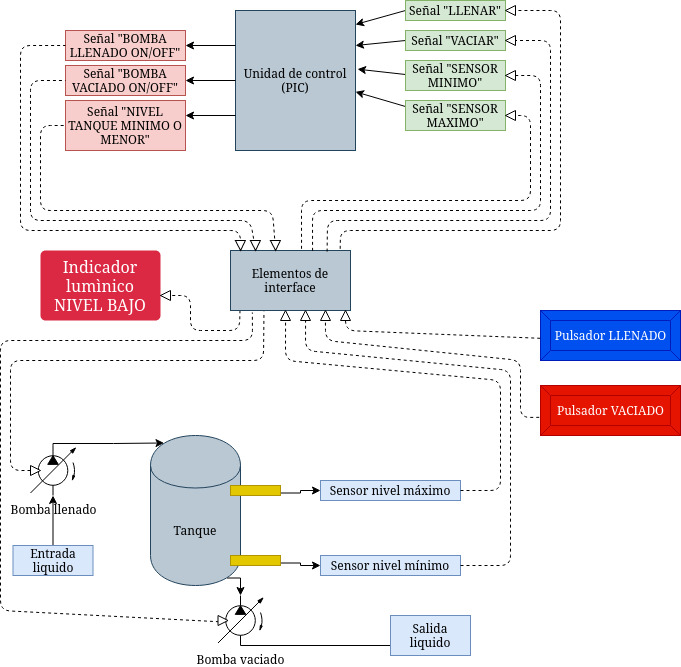
\includegraphics[height=12cm]{diagrama_sistema.jpg}
    \caption{Esquema del sistema general.}\label{fig:esquematico1}
\end{figure}
\clearpage

\subsection{Esquemático del circuito.}

\subsection{Descripción de funcionamiento.}

\section{Análisis y simulación.}

Completar

\section{Conclusiones}

Completar

\noindent\rule{\textwidth}{1pt}

\begin{thebibliography}{9}

\bibitem{bib:compilador}
\textit{``Microchip MPLAB XC8 C Compiler"}
(Versión 2.10; Microchip Technology Inc.: 2019).
Recuperado de https://www.microchip.com/mplab/compilers

\bibitem{bib:simulador}
\textit{``Proteus 8 Professional"} 
(Versión 8.5 Service Pack 0; Labcenter Electronics: 2016).
Recuperado de https://www.labcenter.com/

\bibitem{bid:datasheet}
Microchip (2010).
\textit{``PIC12F629/675 Data Sheet. 8-Pin FLASH-Based 8-Bit CMOS 
Microcontrollers''.}
EE.UU. Recuperado de 
http://ww1.microchip.com/downloads/en/DeviceDoc/41190G.pdf

\end{thebibliography}


\appendix

\section{}
A continuación listamos en extenso el código fuente en lenguaje C
correspondiente al . La descripción de su 
funcionamiento puede encontrarse en la sección de Diseño y 
Simulación.

%\lstinputlisting[language=C,basicstyle=\ttfamily\scriptsize,numbers=left]{../ejercicio1.c}
% `lstinputlisting` inserta el codigo.
% Lo configuro para C, en monospace y tamaño chico, con numeracion a la izquierda.
% Recordar que el archivo tiene una direccion relativa a esta carpeta.
% Los de verdad van a estar en la carpeta padre "../ejercicio1.c"

\newpage
% Incluir salto de pagina de manera manual en cada apendice.
\section{}
A continuación podran ver el  código fuente en lenguaje C correspondiente
al . La descripción de su funcionamiento puede encontrarse en
la sección de Diseño y Simulación.

%\lstinputlisting[language=C,basicstyle=\ttfamily\scriptsize,numbers=left]{../ejercicio2.c}

\end{document}
